\documentclass[9]{beamer}
\usepackage{beamerthemesplit}
\mode<presentation>
{
  \usetheme{Warsaw}
  \setbeamercovered{transparent}
}
%\setbeameroption{show notes}

\usepackage[english]{babel}
\usepackage[latin1]{inputenc}

\usepackage{times}
\usepackage[T1]{fontenc}

% \documentclass{elsart}
% \documentclass[doublespacing]{elsart}
\usepackage{graphicx}
\usepackage[nogin]{Sweave}
\usepackage{amsmath}
\usepackage{amssymb}
\usepackage{yfonts}
\usepackage{amsfonts}
%\usepackage{subfig}
\usepackage{tabls}
\usepackage{url}
\usepackage{pslatex}
\usepackage{makeidx}
\usepackage{dchem}
\usepackage{color}
\usepackage[numbers]{natbib} 
\bibliographystyle{plainnat}

\newcommand{\deriv}[2]{\ensuremath{\frac{\mathrm{d} #1}{\mathrm{d} #2}}}

\title{Statistical Modeling of Biochemical Pathways}
\author{Gregory R. Warnes\inst{1,2,3} }
\institute{ 
  \inst{1}%
  Biostatistics and Computational Biology \\
  University of Rochester
  \and
  \inst{2}%
  Center for Biodefense Immune Modeling \\
  University of Rochester
  \and
  \inst{3}%
  Random Technologies, LLC.
}

\begin{document}

\note{
$ $Id$ $
}


\frame{
  \maketitle
}

%%\section[Abstract]{}
%%\begin{abstract}
%\frame{
%  \frametitle{Abstract}
%    \small
%    We examine the usefulness of Bayesian statistical methods for
%    the modeling of biochemical reactions. With simulated data, it is
%    shown that these methods can effectively fit mechanistic models of
%    sequences of enzymatic reactions to experimental data. This 
%    approach has the advantages of being flexible, relatively easy to use,
%    and producing full probability distributions for the model parameters 
%    rather than point estimates, thus allowing more informative inferences 
%    (including relationships between parameters) to be drawn.  Further,
%    these methods perform well even when the mechanistic model leads 
%    to multiple solution regions, high parameter correlations, and other 
%    'unfriendly' behavior.    

%    The presentation will include a brief overview of Bayesian statistical
%    methods for those unfamiliar with these techniques, as well as a brief
%    discussion of the computational methods utilized.
%}
%%\end{abstract}

\section[Outline]{}
\frame{
  \frametitle{Outline}

%  \tableofcontents

 \begin{columns}
      \begin{column}{0.5\textwidth}
        \tableofcontents[sections={1-4}]
      \end{column}
      \begin{column}{0.5\textwidth}
        \tableofcontents[sections={5-8}]
      \end{column}
    \end{columns}

}

\section{Overview}
\subsection{Goal}
\frame{
  \frametitle{Overview}
  \begin{block}{Goal: Model Biochemical Pathways}
    Estimate key rate parameters of biological pathways, e.g

    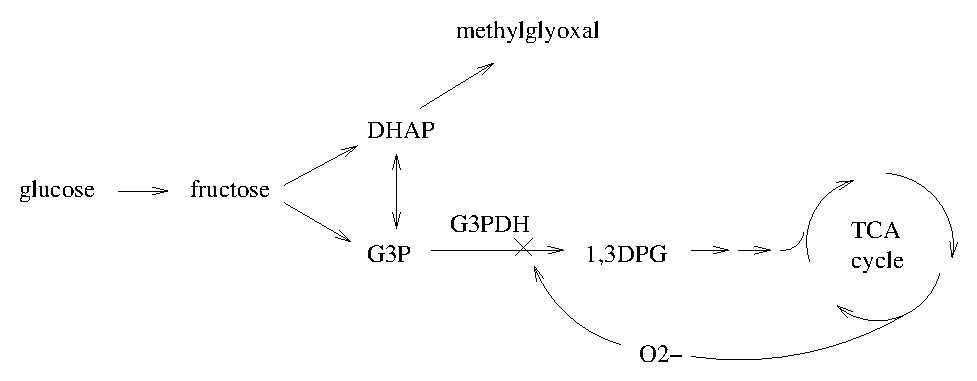
\includegraphics[width=0.75\textwidth]{figures/glycolysis} 

    in order to estimate rate parameters, predict responses to
    changes, and understand the system.
  \end{block}
}

\subsection{Components}
\frame{
  \frametitle{Overview}
  \begin{block}{Combine 3 components:}
    \begin{tabular}{ll}
     Biochemistry        & Biochemical components \& relationships \\
     Mathematical Model  & Strucure of relationships between components \\
     Bayesian Statistics & Relationship between previous information, \\
                         & model and measured data \\
    \end{tabular}

%  \begin{block}{Method:}
%    \begin{center}
%    ``Wrap'' standard deterministic mathematical model describing a
%    biochemical pathway within a Bayesian statistical model 
%    \end{center}
  \end{block}

}  

\subsection{Intro to Bayesian Statistics}
\frame{
  \frametitle{Intro to Bayesian Statistics (1/2)}
  \begin{enumerate}
  \item Based on Decision Theory
  \item Modeling Process:
    \begin{enumerate}
    \item Costruct a model for observed data: {\color{blue} ``Likelihood'':
      $L(\mathit{Data}|\theta)$ }
    \item Describe current information about model parameters:
      { \color{green} ``Prior distribution'' $\pi(\theta)$ }
    \item Run experiment \& collect data
    \item Apply Bayes Rule $\to$ {\color{red}``Posterior distribution''}

\begin{equation}\label{BayesRule}
{\color{red}\pi(\theta|\mathit{Data})} = \frac{{\color{blue}L(\mathit{Data}|\theta)} {\color{green}\pi(\theta)}}{\int {L(\mathit{Data}|\theta) \pi(\theta)}d\theta}
\end{equation}

    \item Draw conclusions using Posterior
    \end{enumerate}
  \end{enumerate}
}

\frame{
  \frametitle{Intro to Bayesian Statistics (2/2)}
  \begin{itemize}
  \item Strengths
    \begin{itemize}
    \item Very flexible
    \item Consistent with human thinking
    \item Allows inclusion of existing domain knowledge
    \end{itemize}
  \item Weaknesses
    \begin{itemize}
    \item Characterization of ``current information'' can be
      controversial
    \item Computationaly expensive 
    \item Less popular than Frequentist statistics
    \end{itemize}
  \end{itemize}
}



\section{Evaluation Approach}

\frame{
  \frametitle{Overview}
  \begin{block}{Goal: Model Biochemical Pathways}
    Estimate key rate parameters of biological pathways, e.g

    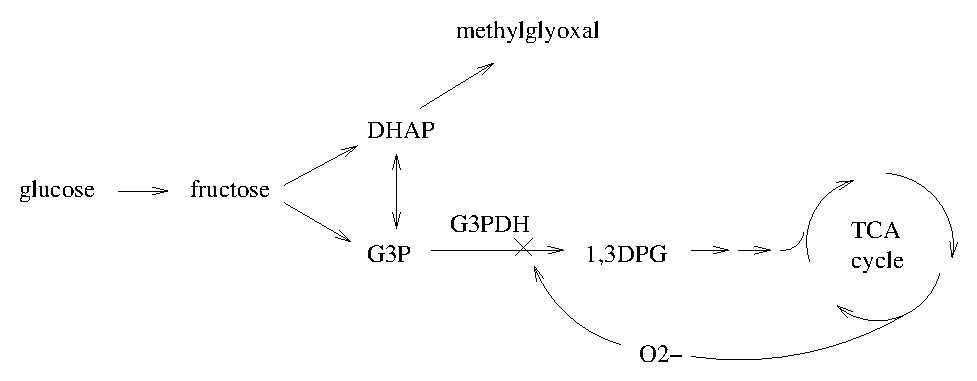
\includegraphics[width=0.75\textwidth]{figures/glycolysis} 

    in order to estimate rate parameters, predict responses to
    changes, and understand the system.
  \end{block}
}


\frame{
  \frametitle{Evaluation Approach}
  \begin{enumerate}
  \item{Create artificial model}
  \item{Generate artificial data}
  \item{Construct Mathematical + Bayesian Model}
  \item{Fit constructed model}
  \item{Compare results to known truth}
  \end{enumerate}
}

\section{Simulation Setup}
\subsection{Pathway Structure}
\frame{
  \frametitle{Pathway Structure}
  Relationship Diagram:
  \begin{reaction} source \yields R1 \yields R2 \yields
    R3 \yields R4 \yields R5 \yields sink \end{reaction}

  Chemical Equations:
  \begin{chemarray*}
    source &\yields^{k_1}& R1\\
    R1 + E1 &\eqbm^{k_2}_{k_3}& R1E1 \yields^{k_4} R2 + E1\\
    R2 + E2 &\eqbm^{k_5}_{k_6}& R2E2 \yields^{k_7} R3 + E2\\
    R3 + E3 &\eqbm^{k_8}_{k_9}& R3E3 \yields^{k_{10}} R4 + E3\\
    R4 + E4 &\eqbm^{k_{11}}_{k_{12}}& R4E4 \yields^{k_{13}} R5 + E4\\
    R5 &\yields^{k_{14}}& sink
  \end{chemarray*}
}

\subsection{Rate constants}
\frame{
  \frametitle{Rate constants}
  \begin{center}
    \begin{tabular}{c|r c c|r}
      rate constant & value & ~ & rate constant & value\\
      \cline{1-2}
      \cline{4-5}
      $k_1$ &  1.600  & ~ &  $k_8$ & 0.090 \\   
      $k_2$ &  0.540  & ~ &  $k_9$ & 4.560 \\   
      $k_3$ & 19.500  & ~ & $k_{10}$ & 1.400 \\
      $k_4$ &  2.125  & ~ & $k_{11}$ & 0.106 \\
      $k_5$ &  0.190  & ~ & $k_{12}$ & 3.670 \\
      $k_6$ &  8.460  & ~ & $k_{13}$ & 1.640 \\
      $k_7$ &  2.077  & ~ & $k_{14}$ & 0.400 \\
      \cline{1-2}
      \cline{4-5}
    \end{tabular}
  \end{center}
}

\subsection{Data Generation}
\frame{
  \frametitle{Data Generation}
  \begin{itemize}
  \item Use Gillespie's method to generate ``observed'' data
  \item Start at equilibrium
  \item Add bolus of $R1$ at time $20$.
    \vspace{-0.125in}
    \begin{center}
      \label{pulse}
      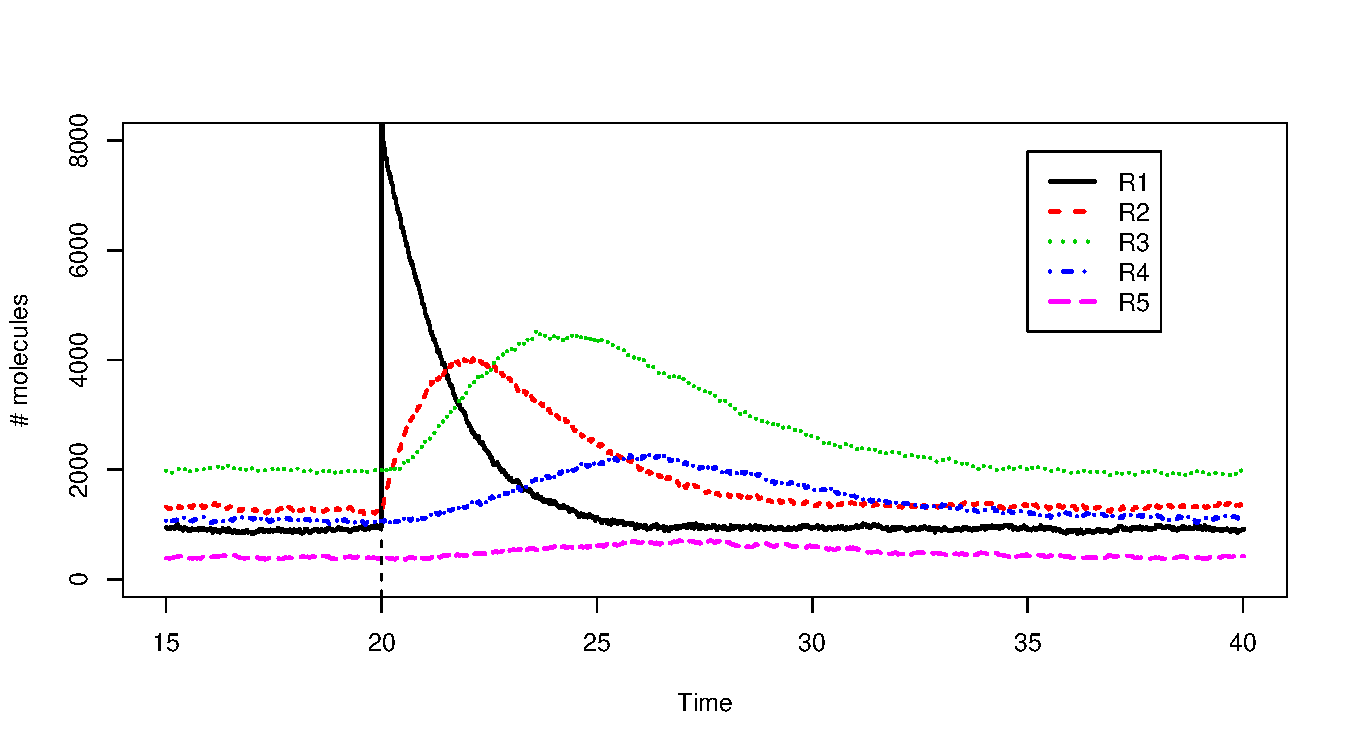
\includegraphics[height=0.6\textheight]{figures/tempDir/pulse}
    \end{center}
    \vspace{-0.125in}
  \item Triplicate estimates of reactant concentrations every minute
  \item Estimate 'velocity' via locally linear smoother, avoiding spike..
  \end{itemize}

}
 
\section{Model Specification}

\subsection{What do we need?}
\frame{
  \frametitle{Model Specification: What do we need?}
  \begin{itemize}
  \item Relationship between parameters and observable data:
    \begin{itemize}
    \item Biochemical model
    \item Error structure
    \end{itemize}
  \item Priors for parameters
  \item Observed Data
  \item Fitting Method
  \end{itemize}
}
 
\subsection{Biochemical Models}
\frame{
  \frametitle{Michaelis-Menten}
  
  Individual reactions were fit using the Michaelis-Menten equation
  for individual enzymes. This is a reaction of the form
  \begin{reaction}\label{eqnForm}
    E + S \eqbm^{k_1}_{k_2} ES \yields^{k_3} E + P
  \end{reaction}
  where
  \begin{eqnarray*}
    S &=& \text{substrate concentration}\\
    E &=& \text{free enzyme concentration}\\
    ES &=& \text{concentration of the enzyme-substrate complex}\\
    P &=& \text{product concentration}
  \end{eqnarray*}
}

\frame{
  \frametitle{Steady State}
    In a steady state the rate
    of the reaction $v$ is
    \begin{equation}
    v = \frac{V_{max}S}{K_m+S} 
    \end{equation}
    where
    \begin{eqnarray*}
      V_{max} &=& (E+ES)k_3 = \text{maximum reaction velocity}\\[2mm]
      K_m &=& \frac{k_2+k_3}{k_1} = \text{substrate concentration at
      half-maximal velocity}
    \end{eqnarray*}
    This form of the equation is very useful because $v$ and $S$ are
    usually measurable and $V_{max}$ and $K_m$ can be obtained by
    fitting  equation 3 to the data. I

    %In contrast, modeling $v$ as a
%    function of the individual rate constants is less useful because
%    that requires the measurement of the concentration of the
%    enzyme-substrate complex which is technically difficult.
}

\frame{
  \frametitle{Non-steady state}
    In this application we are dealing with sequences of reactions
    which are not in a steady state, so we cannot use the
    Michaelis-Menten equation directly. Instead, we use equations
    of the form
    \begin{equation}
    v = \frac{aS}{b+S} - \frac{cP}{d+P} 
  \end{equation}
    
  The coefficients $a$, $b$, $c$, and $d$ in the equations can be
  estimated with data obtained following a change in the
  concentration of one of the reactants. For example, for the data
  plotted in Slide~\ref{pulse}:
    \begin{align*}
      \deriv{R2}{t} &= v_2 = \frac{d_1R1}{d_2 + R1} -
      \frac{d_3R2}{d_4 + R2}\\[5mm]
    \end{align*}
}


\subsection{Error distribution}

\frame{
  \frametitle{Error distribution}
  The error in the velocity estimates is assumed
  to be $N(0,\sigma^2)$ so that the reaction velocities $v_j$ have a
  normal distribution:
  \[
  v_j \sim N(\mu_j,\sigma^2)
  \]

  where
  \[
  \mu_j = \frac{aS_j}{b+S_j} - \frac{cP_j}{d+P_j} 
  \]
}

\frame{
  \frametitle{Likelihoods}
  Putting this together yields:
  \begin{align*}
    v_2 &\sim N\left(\frac{d_1R1}{d_2+R1} -
      \frac{d_3R2}{d_4+R2}, \;\; \sigma^2\right)\\
    v_3 &\sim N\left(\frac{d_3R2}{d_4+R2} -
      \frac{d_5R3}{d_6+R3}, \;\; \sigma^2\right)\\
    v_4 &\sim N\left(\frac{d_5R3}{d_6+R3} -
      \frac{d_7R4}{d_8+R4}, \;\; \sigma^2\right)\\
    \intertext{and}
    v_5 &\sim N\left(\frac{d_7R4}{d_8+R4} - d_9R5, \;\; \sigma^2\right)
  \end{align*}
}

\subsection{Prior Distributions}

\frame{
  \frametitle{Prior Distributions}

  For coefficients $d_1$ -- $d_5$: 
  \[
  \frac{3d_i}{\mu_i} \sim \chi_5^2
  \]
  where $\mu_i$ is a prior estimate of the parameter values.
  
  ~ 

  For $\sigma^2$:
  \[
  \sigma \equiv 2
  \]
  }

\section{Fitting}
\frame{
  \frametitle{Fitting algorithm}
  
  We applied 3 different MCMC algorithms (in order of shortest to
  longest required run length) as implemented in the \textsc{Hydra}
  MCMC library for \textsc{Java}.

  \begin{enumerate}
    \item Normal Kernel Coupler
    \item Multivariate normal increment Metropolis
    \item Univariate normal increment Metropolis
  \end{enumerate}
  
  Convergence and required run-length was estimated using
  \textsc{mcgibbsit}, using $q=0.025$, $r=0.0125$, and $s=0.95$,
  which ensure reliable confidence intervals. 
}

\frame{
\begin{block}{What is Markov Chain Monte Carlo?}

\textcolor{blue}{Markov Chain Monte Carlo (MCMC)} is a technique for
generating \textcolor{red}{dependent} samples (a Markov Chain) from a
distribution without needing the \textcolor{blue}{normalizing constant}.

\end{block}
\begin{block}{When is MCMC useful?}

\textcolor{blue}{MCMC} is useful when it is \textcolor{red}{difficult} to
\textcolor{blue}{simulate} from the target distribution, such as when the
\textcolor{blue}{normalizing constant} is difficult or impossible to
compute and \textcolor{blue}{rejection sampling} is not possible.

Examples:
\begin{itemize}
  \item Sampling from \textcolor{blue}{Bayesian Posterior Distributions}
  \item Computing \textcolor{blue}{Maximum-Likelihood tests for intractable
    likelihoods}
\end{itemize}

\end{block}

}

\frame{
\frametitle{MCMC In pictures}
\begin{center}
\includegraphics[height=0.75\textheight]{MCMC-Picture}
\hfill
\includegraphics[height=0.75\textheight]{MCMC-Histogram}
\end{center}
}


\frame{
  \frametitle{Convergence Rates (1/2)}
  \begin{center}
    Mean Squared Residuals \\
    ~

    \begin{tabular}{c||c|c|c||c|c|c}
       &
       \multicolumn{3}{c||}{mean residual SSQ $\times 10^{-4}$} & \multicolumn{3}{c}{$R_{adj}^2$}\\
      \cline{2-7}
      algorithm & 12 pt. & 16 pt. & 25 pt. &
      12 pt. & 16 pt. & 25 pt.\\
      \hline
       1-comp & 1.34 & 0.83 & 1.06 & 0.87 & 0.92 & 0.86\\
       all-comp & 0.74 & 0.93 & 0.74 & 0.93 & 0.90 & 0.90 \\
       NKC & 0.86 & 0.73 & 0.71 & 0.92 & 0.92 & 0.91
    \end{tabular}
  \end{center}
}

\frame{
  \frametitle{Convergence Rates (2/2)}
  \begin{center}
    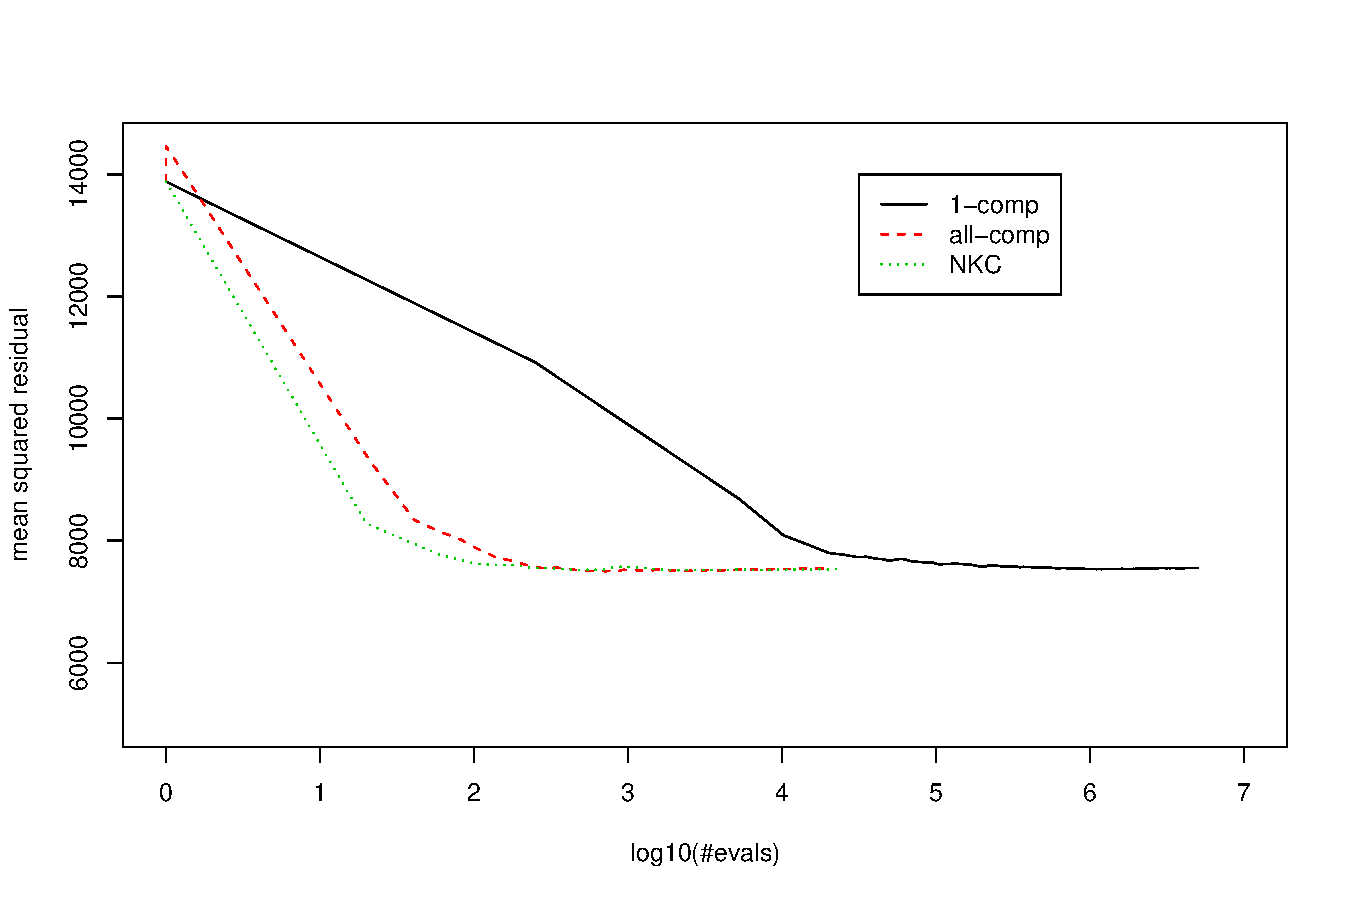
\includegraphics[scale=0.5]{figures/MSR16}
  \end{center}


}


\section{Results}
\frame{
  \frametitle{Results}
  
  
  \begin{columns}[c]
  \column{2in} 

  Bivariate scatter plots of the parameter distributions (upper
  triangle) and correlation coefficients (lower triangle). 

  ~

  Note the strong correlation between some pairs of parameters,
  e.g., $d_1$ -- $d_2$.

  \column{2in}

  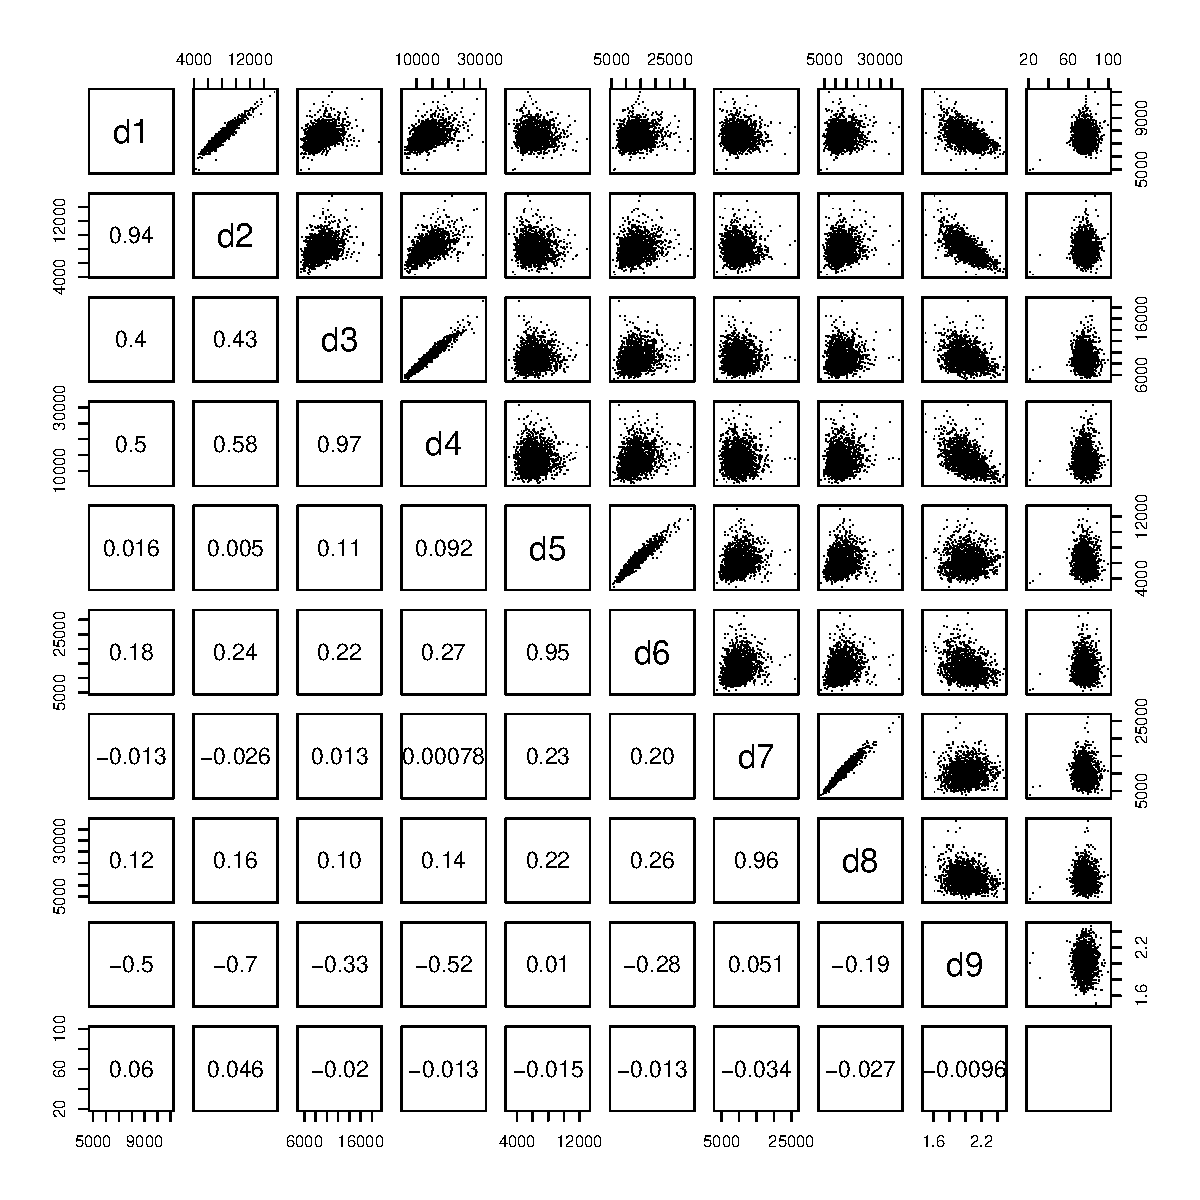
\includegraphics[width=2in]{figures/tempDir/scatterPlot}
  \end{columns}
}

\frame{
  \frametitle{Actual vs Fitted}

  \begin{center}
  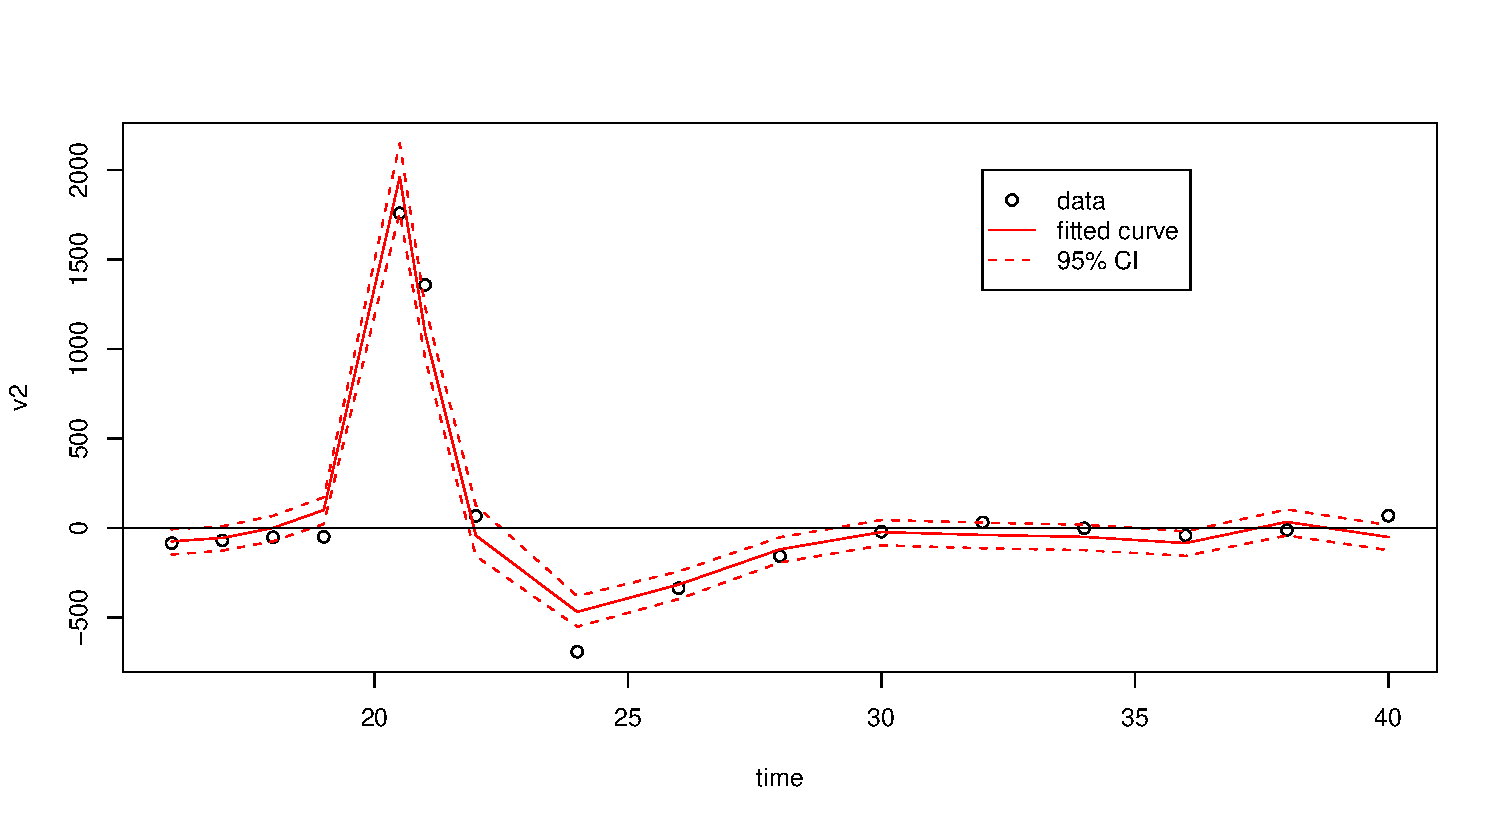
\includegraphics[width=0.5\textwidth]{figures/tempDir/V1fitted}
  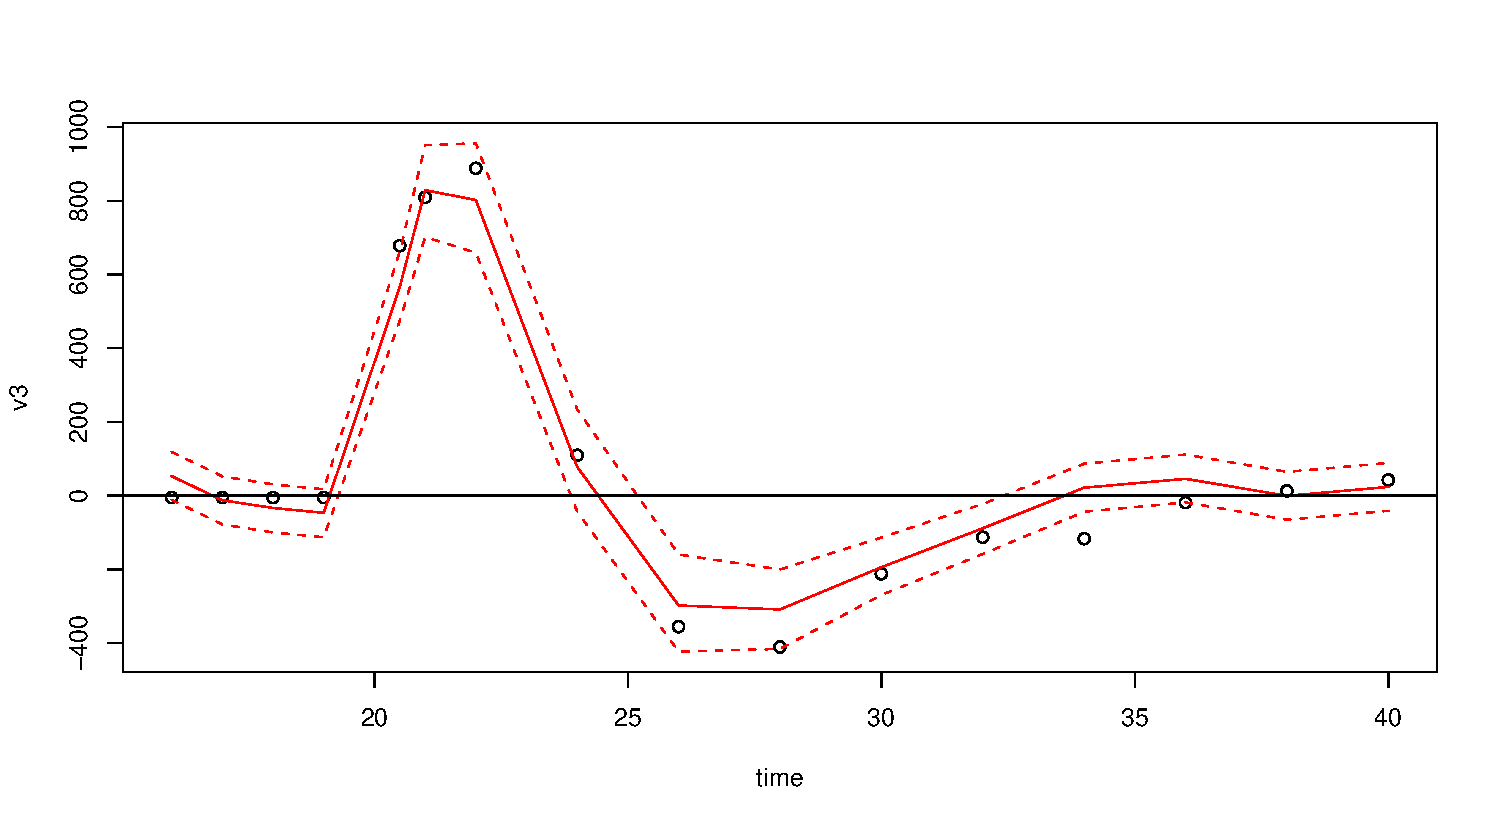
\includegraphics[width=0.5\textwidth]{figures/tempDir/V2fitted} \\

  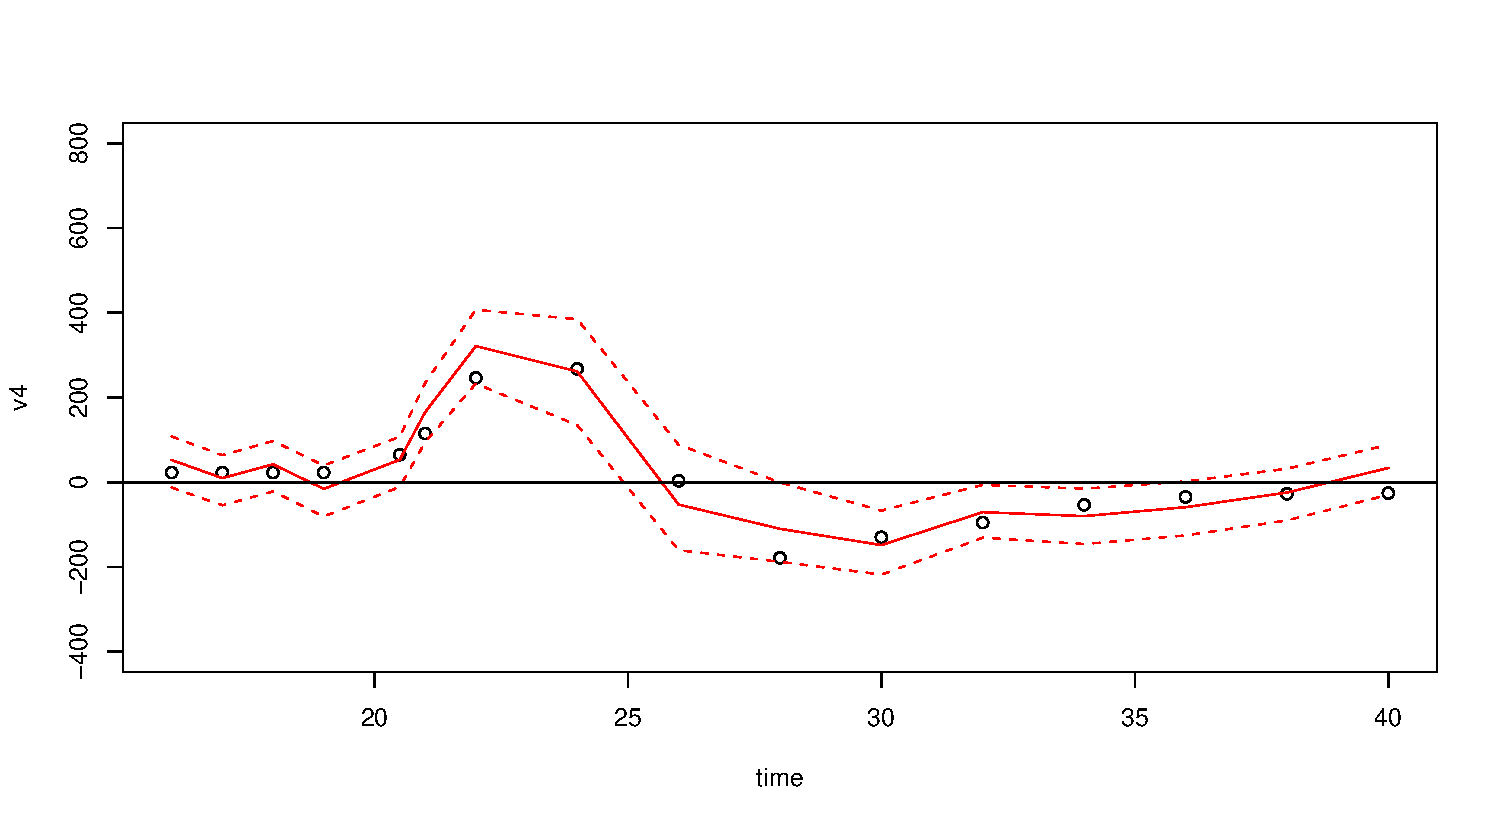
\includegraphics[width=0.5\textwidth]{figures/tempDir/V3fitted}
  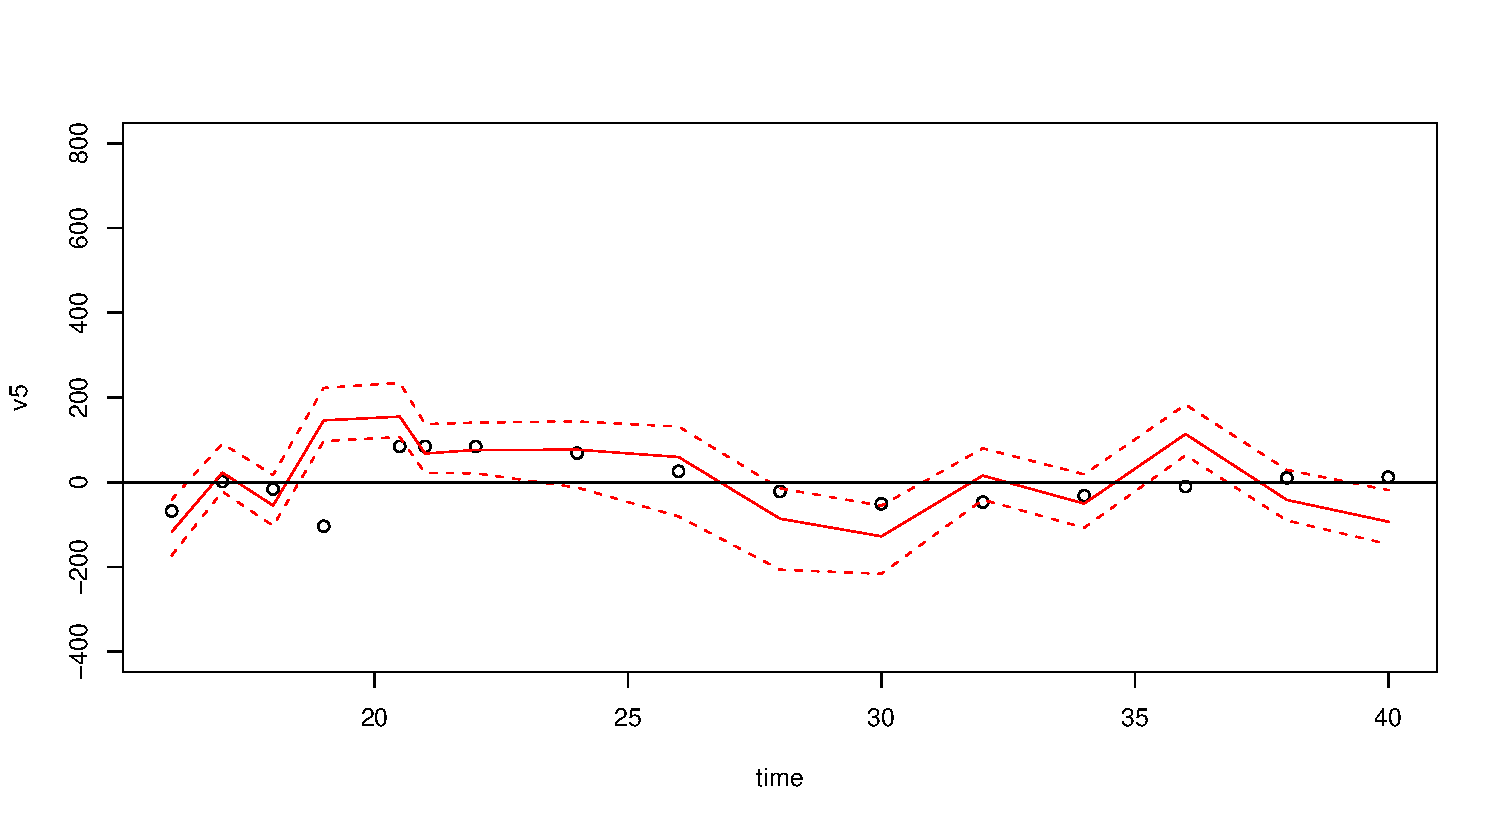
\includegraphics[width=0.5\textwidth]{figures/tempDir/V4fitted} \\
  \end{center}
}

\section{Acknowledgments}
\frame{
  \frametitle{Acknowledgments}

  Robert "Bing" Burrows, Ph.D., who was primarily responsible for work
  described here passed away unexpectedly on December 27, 2006.

\begin{quote}
\tiny
  BURROWS, ROBERT BERNARD, II, 63, of North Scituate [Rhode Island],
  died Wednesday, December 27, 2006. He was a long time resident of
  Lexington, MA before moving to Rhode Island in 2001. After
  graduating from Lexington High School, Dr. Burrows earned his
  Bachelor of Arts from Northeastern University, a Ph.D. in
  Biochemistry from the Massachusetts Institute of Technology, and a
  Master of Science in Statistics from the University of Rhode Island.
  He was a self-employed Research Biochemist and previously worked for
  the Boston Biomedical Research Institute. He leaves his sister Ellen
  Conner and her husband Donald of Coventry, his dearest friend Sally
  Glanz of North Scituate and many cousins. (\emph{The Providence Journal/Evening
      Bulletin} 2006 Dec. 31; Sec. B5)
\end{quote}
}

\section[]{Reference \& Contact Information}
\frame{
  \frametitle{Reference \& Contact Information}
  \begin{block}{Manuscript}
    Burrows~RB, Warnes~GR, Hanumara~RC, ``Statistical Modeling of Biochemical Pathways'',
    \emph{IET Systems Biology}, IET Syst. Biol. 1, 353 (2007)
  \end{block}
  \begin{block}{Contact Information}
    \begin{itemize}
    \item Email:              \texttt{greg@warnes.net}
    \item Personal Web Page:  \texttt{http://www.warnes.net}
    \item CBIM Web Page:      \texttt{https://cbim.urmc.rochester.edu}
    \item UR Biostat Web Page \texttt{http://www.urmc.rochester.edu/smd/biostat}
    \end{itemize}
  \end{block}
}

%%\bibliography{./refs}
%\begin{thebibliography}{99}
%  \bibitem{Oates02}%1
%    Oates,~P.J., 2002, Polyol pathway and diabetic peripheral
%    neuropathy, \emph{Int. Rev. Neurobiol.},
%    \textbf{50}, 325--392.
%  \bibitem{Gilks95} %5
%    Gilkes,~W.R., Richardson,~S., and Spiegelhalter,~D.J. (Ed.),
%    \emph{Markov Chain Monte Carlo in Practice} (Boca Raton, FL:
%    Chapman \& Hall/CRC)
%  \bibitem{R}%9
%    R Development Team, \emph{R: A Language and Environment for
%    Statistical Computing}, http://www.r-project.org (accessed 7 Nov 06)
%  \bibitem{Michaelis13} %10
%    Michaelis, L. and Menten, M.L., 1913, Die kinetic der
%    invertinwirkung, \emph{Biochem. Zeit.}, \textbf{49},
%    333--369.
%  \bibitem{Hydra}%13
%    Warnes, G.R., Hydra {MCMC} {L}ibrary,
%    http://www.sourceforge.net/projects/hydra-mcmc 
%  \bibitem{Warnes00} %14
%    Warnes, G.R., 2000, The {N}ormal {K}ernel {C}oupler: {A}n adaptive
%    {M}arkov chain {M}onte {C}arlo method for efficiently sampling
%    from multi-modal distributions, thesis, University of Washington.
%  \bibitem{projo}%16
%    OBITUARIES-SCITUATE-BURROWS. \emph{The Providence Journal/Evening
%      Bulletin} 2006 Dec. 31; Sec. B5
%\end{thebibliography}




\end{document}
